\documentclass{article}

% LaTeX Packages
\usepackage[letterpaper, total={6.5in, 9in}]{geometry}
\usepackage{graphicx}
\usepackage{layout}
\usepackage{relsize}
\usepackage{lipsum}
\usepackage{ncar_branding} % initialize ncar_branded package here, perhaps with options, or beamer will do it later

\renewcommand{\familydefault}{\sfdefault} % prefer sans-serif fonts (yuck, I think)


\begin{document}

\title{This is my title}
%\subtitle{and I might have a subtitle too!}
\author{Author One, Author Two}
\maketitle

\begin{abstract}
  \lipsum[1]
\end{abstract}

\section{First Section}
\lipsum[1]
\begin{figure}
  \centerline{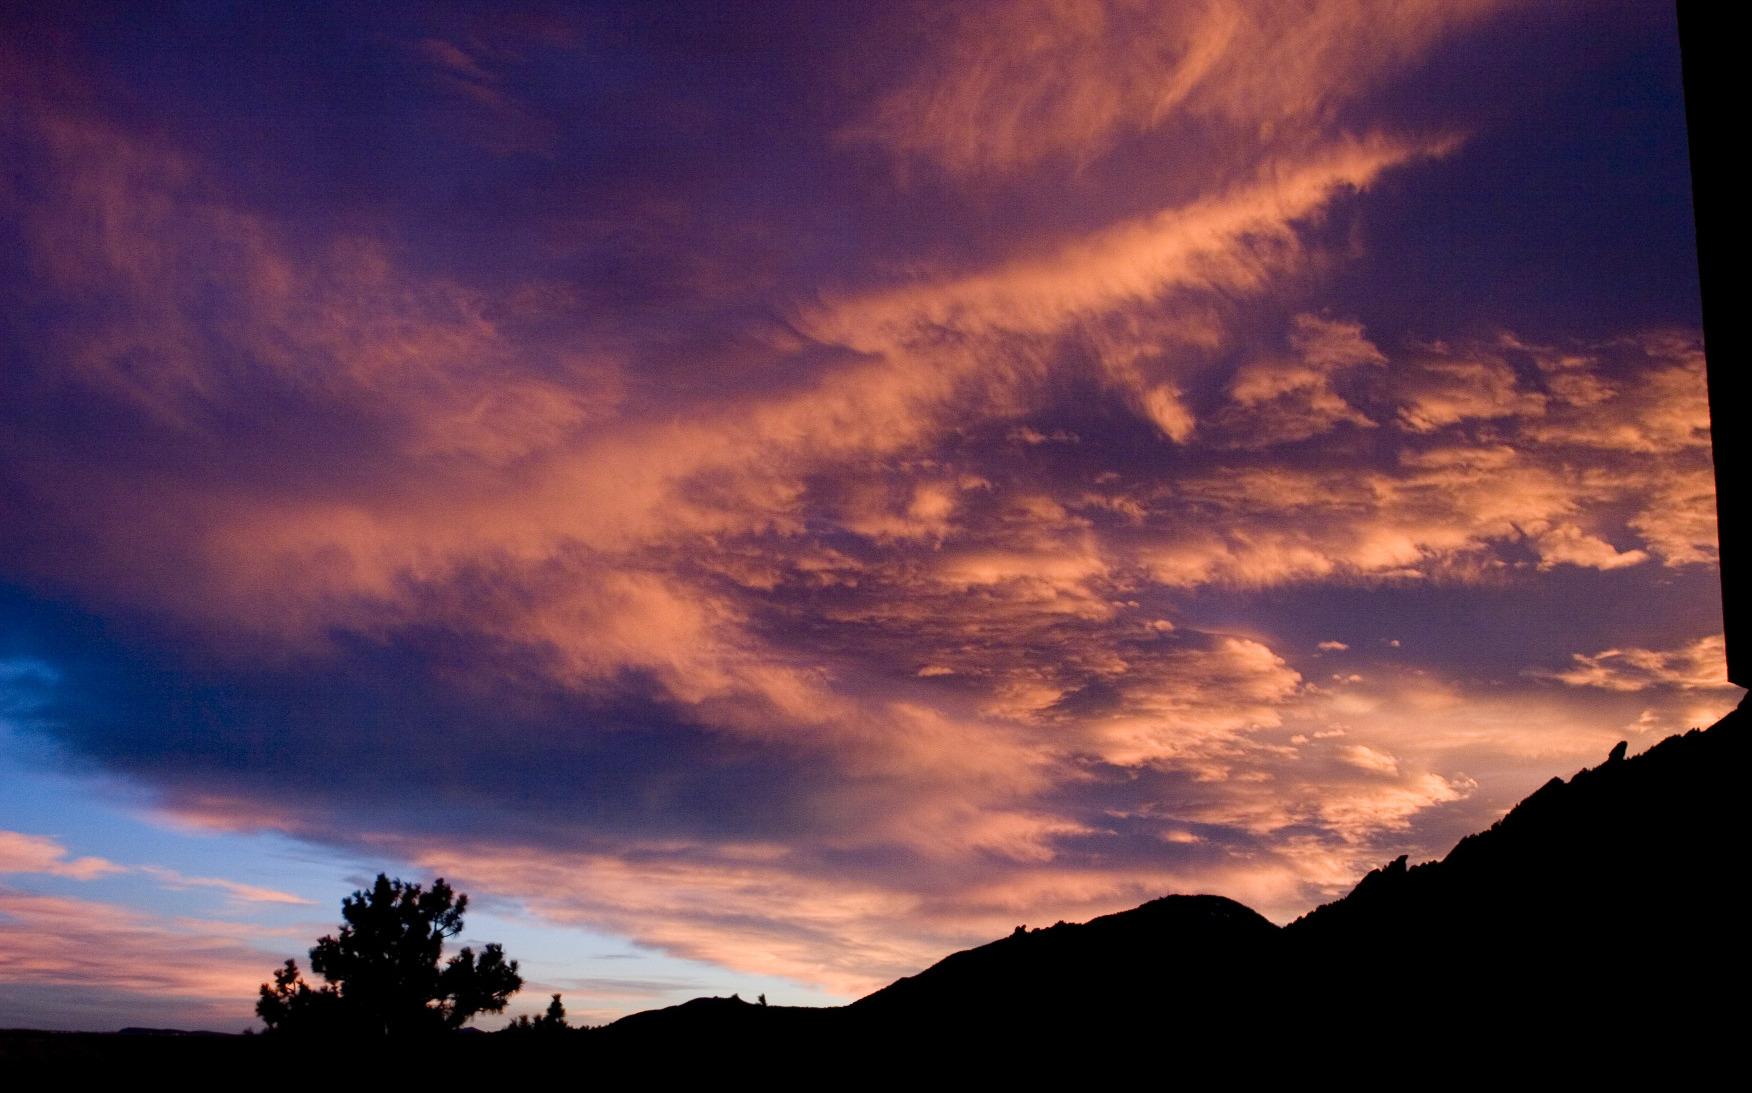
\includegraphics[width=0.5\textwidth]{common/images/wallpaper/mesa_lab_sunset}}
  \caption{Pretty Picure.\label{fig:pretty}}
\end{figure}
Reference my pretty picture (Figure~\ref{fig:pretty}).

\subsection{Subsection}
\lipsum[2]
\begin{equation}
  \frac{\partial \rho}{\partial t} +
  \frac{\partial}{\partial x_{j}} (\rho u_{j}) = 0
\end{equation}
\begin{equation}
  \frac{\partial}{\partial t} (\rho u_{i}) +
  \frac{\partial}{\partial x_{j}} (\rho u_{i} u_{j} + p \delta_{ij} - \tau_{ji} )
  = 0
\end{equation}
\begin{equation}
  \frac{\partial}{\partial t} ( \rho e_{0} ) +
  \frac{\partial}{\partial x_{j}}
  ( \rho u_{j} e_{0} + u_{j} p + q_{j} - u_{i} \tau_{ij} ) = 0
\end{equation}
\lipsum[3]

\section{Second Section}
\lipsum[4]
\subsection{Sample Code}

\subsubsection{Sample Python Code}
\lstinputlisting[language=Python]{snippets/hello_world_mpi4py.py}

\subsubsection{Sample C++ Code}
\lstinputlisting[language=C++]{snippets/hello_world.cxx}

\section{Conclusion}
\lipsum[5-6]
\clearpage
\layout

\end{document}
